\documentclass[11pt,twocolumn]{article}
\usepackage[utf8]{inputenc}
\usepackage{amsmath}
\usepackage{amssymb}
\usepackage{graphicx}
\usepackage{booktabs}
\usepackage{hyperref}
\usepackage{geometry}
\usepackage{natbib}
\usepackage{pgfplots}
\pgfplotsset{compat=1.18}
\geometry{a4paper, margin=0.75in}

\title{\textbf{Identity-Tracked, Boundary-Escalating Sparsity:\\A General Failure Mode in Distributional SAE Regularizers, and a Fix}}
\author{William Knott\\}
\date{Draft --- August 2026}

\begin{document}

\maketitle

\begin{abstract}
Sparse Autoencoders (SAEs) trained with $L_1$ regularization suffer from \textit{shrinkage}: the penalty is paid directly on activation magnitude, so gradient descent shrinks true feature strength toward zero rather than paying the reconstruction cost of leaving it intact \citep{wright2024addressing}. We identify a general failure mode in the natural family of shrinkage-free alternatives to $L_1$: objectives that penalize the \emph{shape} of the activation distribution (e.g.\ a Gini-coefficient penalty) rather than magnitude directly. Such objectives are permutation-invariant over feature identity and have \emph{vanishing gradient at their own degenerate optimum} -- the uniform-activation state where a single feature fires on nearly every input. We demonstrate this concretely using the Gini coefficient as a case study: at matched sparsity, Gini-regularized SAEs initially appear to strongly outperform a sparsity-matched Top-$k$ SAE on causal feature-steering metrics ($1.3$--$2.8\times$, replicated across three datasets), but this is an artifact of exactly the predicted failure -- Gini reliably collapses onto a handful of polysemantic ``hub'' features (class-purity $\approx 0$) rather than genuinely selective ones. Two natural repairs, each targeting one half of the problem, fail for the same underlying reason. A second distribution-shape measure (the Theil index) shows the identical failure, confirming the mechanism generalizes beyond Gini specifically. We propose a general fix -- objectives that track \emph{identity-level} statistics (a specific feature's own firing rate, persistent across the batch) with gradients that \emph{escalate}, not vanish, near the degenerate state -- and instantiate it as Rate-KL, a per-feature KL-divergence penalty on firing probability that never touches magnitude. A second, functionally unrelated instantiation of the same two properties (an interior-point log-barrier penalty) shows the same benefit, indicating the design principle, not the specific KL formula, is what matters. We position Rate-KL explicitly against Top-$k$, Gated SAEs, and Tuned $L_1$ on monosemanticity, steering impact, and reconstruction fidelity: it produces the most class-selective high-importance features and the highest steering impact of any method tested at its best operating point, at the worst reconstruction fidelity of any method tested, including the flawed Gini baseline -- a real, quantified cost we report rather than obscure.
\end{abstract}

\section{Introduction}
Sparse Autoencoders decompose neural network activations into features intended to be sparse and causally meaningful. The dominant recipe penalizes an $L_1$ norm on the latent code. Because this penalty is paid directly on magnitude, \citet{wright2024addressing} show SGD finds it cheaper to shrink a feature's true strength toward zero -- \textit{shrinkage} -- than to pay the reconstruction cost of leaving a legitimately large, sparse feature intact. Gated SAEs \citep{lieberum2024gated}, JumpReLU \citep{rajamanoharan2024jumprelu}, and Top-$k$ SAEs \citep{gao2024topk} each fix this architecturally, by decoupling ``does this feature fire'' from ``how large is it when it fires,'' at the cost of added machinery (a gate, a learned threshold, a hard selection with a straight-through estimator).

This paper is about a different, purely objective-level route to the same goal, and a general failure mode we found in it. Distributional sparsity measures -- of which the Gini coefficient is a well-established example, with an established pedigree in compressive sensing \citep{hurley2009comparing, zonoobi2011gini} -- are scale-invariant by construction: they penalize the \emph{shape} of the activation distribution, never its scale, so they are natural shrinkage-free candidates that need no architectural change. We show this entire family shares a structural weakness that is not specific to any one measure: such penalties are computed after discarding \emph{which} feature produced which value (via sorting, or any other permutation-invariant reduction), and their gradient vanishes exactly at the degenerate point -- uniform activation -- that a ``hub'' feature (one that fires on nearly every input) occupies. An objective built this way cannot push itself away from a hub once one forms, because the hub sits at a flat region of the loss landscape.

We demonstrate this using the Gini coefficient as a concrete instrument, not because Gini is uniquely flawed, but because it is the cleanest available case study: it is fully differentiable, has no other moving parts, and its initial result is dramatic enough to make the subsequent diagnosis legible.

\begin{enumerate}
\item At matched sparsity, Gini-optimized SAEs substantially outperform a sparsity-matched Top-$k$ SAE on steering-impact metrics, replicated across three datasets and three seeds (Section \ref{sec:initial-result}).
\item This is an artifact of the general failure mode above: Gini reliably collapses onto a small number of reused ``hub'' features carrying disproportionate causal weight while being almost maximally class-promiscuous (Section \ref{sec:diagnosis}).
\item Two structurally motivated repairs -- usage-balancing (an MoE load-balancing analogue \citep{shazeer2017outrageously, fedus2022switch}) and a column-wise Gini term that does track feature identity -- each fix one half of the pathology while breaking the other, confirming that identity-tracking alone is insufficient without also fixing the vanishing-gradient problem (Section \ref{sec:failed-fixes}). A second distribution-shape measure, the Theil index, shows the identical hub signature (Section \ref{sec:theil}), confirming the failure mode is not Gini-specific.
\item This motivates a general design principle -- objectives should be \emph{identity-tracked} and \emph{boundary-escalating} -- instantiated as Rate-KL, a per-feature firing-rate penalty with no magnitude term at all (Section \ref{sec:ratekl}). A second, functionally unrelated instantiation (a log-barrier penalty, Section \ref{sec:barrier}) shows the same qualitative benefit, indicating the principle generalizes beyond the specific KL formula. We position Rate-KL explicitly against Top-$k$, Gated SAEs, and Tuned $L_1$ on monosemanticity, steering, and fidelity (Section \ref{sec:positioning}), and report an honest, real fidelity cost.
\end{enumerate}

\section{Related Work}
\label{sec:related}
Our approach sits between structural sparsity mechanisms (Top-$k$ SAEs \citep{gao2024topk}) and magnitude-based regularizers ($L_1$, KL-sparsity autoencoders). \citet{hurley2009comparing} establish the Gini index as satisfying all six axiomatic requirements of a sparsity measure, unlike $L_1$; its use as a differentiable \emph{training} penalty, rather than a post-hoc measure, is comparatively unexplored, and to our knowledge its specific failure mode on SAE latents has not been previously characterized. Gated SAEs \citep{lieberum2024gated} and JumpReLU \citep{rajamanoharan2024jumprelu} address shrinkage architecturally; Top-$k$ SAEs \citep{gao2024topk} avoid it by applying no magnitude penalty and using hard per-sample selection instead. Our usage-balancing fix attempt is a direct analogue of Mixture-of-Experts load-balancing losses \citep{shazeer2017outrageously, fedus2022switch}, which solve the structurally identical problem of the same experts being selected for every input. \citet{chanin2024absorption} identify \emph{feature absorption} -- a concept's dedicated latent developing activation holes because a co-occurring, more specific latent has absorbed its direction -- as a distinct sparsity-induced failure mode from the hub pathology we diagnose here; we tested Rate-KL against a class-level adaptation of their metric but our evaluation proxy was not sound enough on two of three datasets to support a claim in either direction (Section \ref{sec:limitations}). Classic KL-sparsity autoencoders \citep{ng2011sparse} penalize a feature's mean \emph{activation}, which -- unlike our firing-rate formulation -- is itself a magnitude-suppressive, $L_1$-like penalty in disguise.

\section{A General Failure Mode: Distribution-Shape Sparsity Objectives}
\label{sec:method-gini}
Consider any sparsity penalty $\Phi(z)$ computed from a latent code $z \in \mathbb{R}^n$ via a statistic that is (a) invariant to which index produced which value (e.g.\ computed from the \emph{sorted} values, as any dispersion or inequality measure is), and (b) has vanishing gradient at its own degenerate optimum. We claim any such $\Phi$ is structurally exposed to the hub pathology diagnosed in this paper, independent of the specific functional form. Property (a) means the objective has no mechanism to prefer \emph{which} features carry its distributional mass, only that some do; property (b) means that once a feature becomes a hub, the objective cannot generate gradient to correct it. The Gini coefficient is one instance of this family; Section \ref{sec:theil} confirms the same failure in a second, structurally different instance (the Theil index), and we expect it to recur in other permutation-invariant dispersion measures applied the same way.

For a latent code $z$, the Gini coefficient admits a differentiable rank-based formulation,
\begin{equation}
G(z) = \frac{2 \sum_{i=1}^n i \cdot z_{(i)}}{n \sum_{i=1}^n z_{(i)}} - \frac{n+1}{n},
\label{eq:gini}
\end{equation}
where $z_{(i)}$ are absolute activations sorted ascending via \texttt{torch.sort}, gradients routed to original positions via the inverse permutation. $G$ is scale-invariant ($G(\alpha z){=}G(z)$, $\alpha{>}0$): an active neuron that ``shouts'' above the rest is \emph{rewarded}, since it increases inequality. Training minimizes $\mathrm{MSE} - \lambda\,\mathbb{E}[G(z)]$, pushing toward high-inequality activations with no pressure on the scale of the surviving values.

\subsection{Initial Result: Gini Beats Matched-Sparsity Top-$k$}
\label{sec:initial-result}
We trained Gini and Top-$k$ SAEs (Top-$k$'s $k$ set to Gini's observed mean active count) on MNIST, Fashion-MNIST, and CIFAR-10, three seeds each, $N{=}1024$, and measured mean active-feature magnitude and steering impact (feature ablation and $3\times$ clamping, averaged over 1000 sample-feature interventions).

\begin{table}[h]
\centering
\caption{Gini vs.\ sparsity-matched Top-$k$, mean over 3 seeds. Sparsity matched to within 0.2pp on every dataset.}
\label{tab:initial-result}
\begin{tabular}{@{}lccc@{}}
\toprule
Dataset & Magnitude & Ablate & Clamp \\
& (ratio) & (ratio) & (ratio) \\ \midrule
MNIST & $2.52\times$ & $1.96\times$ & $1.96\times$ \\
Fashion-MNIST & $2.80\times$ & $1.88\times$ & $1.88\times$ \\
CIFAR-10 & $1.76\times$ & $1.27\times$ & $1.27\times$ \\ \bottomrule
\end{tabular}
\end{table}

The effect replicates cleanly and shrinks with dataset complexity, alongside a shrinking MSE penalty (66\% worse than Top-$k$ on MNIST, 43\% on Fashion-MNIST, 3\% on CIFAR-10). Taken at face value, this is striking: a purely distributional penalty outperforming the current default shrinkage-free method. Section \ref{sec:diagnosis} shows why it should not be.

\subsection{Diagnosis: The Hub-Feature Pathology}
\label{sec:diagnosis}
For each active feature we compute its exact ablation-impact norm ($|z_f|\cdot\lVert W_{\mathrm{dec}}[:,f]\rVert_2$, closed-form for a linear decoder) summed over the test set as total causal \emph{importance}, and its class-purity: $1 - H(y\mid f\text{ active})/\log_2(10)$ (1.0 = fires for exactly one class; 0.0 = uniform across all ten).

\begin{table}[h]
\centering
\caption{Importance concentration and class purity, Fashion-MNIST, one seed. Top-10\% is by importance.}
\label{tab:diagnosis}
\begin{tabular}{@{}lcccc@{}}
\toprule
Model & Imp.\ Gini & Top-10\% & Mean & Top-10\% \\
 & coeff.\ & share & purity & purity \\ \midrule
Gini & 0.768 & 67.2\% & 0.150 & \textbf{0.001} \\
Top-$k$ & 0.576 & 41.3\% & 0.278 & 0.036 \\
Gated & 0.522 & 37.7\% & 0.093 & 0.003 \\
Tuned $L_1$ & 0.370 & 26.1\% & 0.053 & 0.000 \\ \bottomrule
\end{tabular}
\end{table}

Gini's importance is far more concentrated than Top-$k$'s (67\% in the top decile vs.\ 41\%), and the features carrying it are essentially maximally class-promiscuous (purity 0.001) -- indistinguishable from firing uniformly across every class. Gini's mean purity (0.150) is roughly half of Top-$k$'s (0.278). Table \ref{tab:initial-result}'s steering advantage is driven almost entirely by generic hub directions, not restored-magnitude monosemantic concepts, exactly as predicted by property (b) above. A downstream-consequence check confirms the artifact is not confined to the reconstruction-internal metric: clamping a hub feature and measuring the resulting flip rate of a linear classifier on the frozen latents replicates the pattern (Gini: 8.1\% clamp flip rate vs.\ Top-$k$'s 3.5\%).

\subsection{Two Failed Fixes and Their Shared Cause}
\label{sec:failed-fixes}
\textbf{Usage-balancing.} Penalizing usage concentration directly, $\mathrm{bal}(z) = n\sum_f p_f^2$ ($p_f$ = feature $f$'s share of batch activation mass, an MoE-style Herfindahl term \citep{shazeer2017outrageously,fedus2022switch}), fixes purity decisively at $\lambda_{\mathrm{bal}}{=}0.01$ (top-decile purity $0.001\to0.171$, above Top-$k$'s $0.036$, matched sparsity, unchanged MSE) but collapses steering to \emph{below} Top-$k$'s ($0.041$ vs.\ $0.090$ ablate, $\approx45\%$ of Top-$k$'s level). Per-occurrence steering impact is $|z_f|\cdot\lVert W_f\rVert$ when a feature fires; forcing usage toward uniform mathematically forbids features from being rare-but-strong, which is exactly what maximizes that quantity. We optimized directly against the thing we wanted to win on.

\textbf{Column-wise Gini.} A hub is a column of the latent matrix $Z$ that is uniformly large across the batch -- low column-Gini; a selective feature has high column-Gini. Maximizing $G$ along both axes ($\mathcal{L} = \mathrm{MSE} - \lambda_{\mathrm{row}}\mathbb{E}[G(\mathrm{rows})] - \lambda_{\mathrm{col}}\mathbb{E}[G(\mathrm{cols})]$) does track identity per-feature -- yet fails outright: top-decile purity barely moves ($0.001\to0.013$ at $\lambda_{\mathrm{col}}{=}0.3$), sparsity drifts far off-target (to 0.98), and MSE more than doubles. A hub column sits \emph{exactly} at $G{=}0$, its own degenerate point, where the Gini gradient is flat (verified directly: a synthetic uniformly-active column has near-zero gradient vs.\ $G{=}0.969$ and strong gradient for a selective column). Averaged over 1024 features, SGD takes the cheap escape -- nudging 900 already-marginal columns slightly more selective raises the mean at negligible cost, while fixing an actual hub is expensive.

Both failures confirm the same lesson from different sides. Usage-balancing has identity but the wrong target statistic; column-Gini has the right statistic but the wrong gradient shape at the point that matters. Identity-tracking alone is not sufficient -- the gradient must also escalate, not vanish, at the degenerate point.

\subsection{A Second Instance: The Theil Index}
\label{sec:theil}
Section \ref{sec:method-gini} claims the hub pathology is a property of the class of permutation-invariant, vanishing-gradient-at-degeneracy objectives, not specific to Gini. We test this with the Theil index, a differently-shaped generalized-entropy inequality measure ($T(x) = \frac{1}{n}\sum_i \frac{x_i}{\bar x}\log\frac{x_i}{\bar x}$, minimized at $T{=}0$, the uniform-activation hub state). A gradient check confirms the same structural weakness before any training: on a synthetic hub vector, Theil's gradient norm is $3.7{\times}10^{-9}$; on a genuinely varied selective vector, $0.094$ -- the identical vanishing-gradient-at-degeneracy signature as Gini.

\begin{table}[h]
\centering
\caption{Theil-regularized SAE vs.\ Top-$k$, Fashion-MNIST, one seed.}
\label{tab:theil}
\begin{tabular}{@{}lccc@{}}
\toprule
Model & Sparsity & Mean purity & Top-10\% purity \\ \midrule
Theil ($\lambda{=}0.0005$) & 0.629 & 0.170 & \textbf{0.0003} \\
Theil ($\lambda{=}0.001$) & 0.679 & 0.188 & \textbf{0.0002} \\
Top-$k$ (ref.) & \textbf{0.910} & \textbf{0.348} & 0.023 \\ \bottomrule
\end{tabular}
\end{table}

Top-decile purity is essentially zero for Theil ($0.0002$--$0.0003$, lower even than Gini's own $0.001$) and mean purity is roughly half of Top-$k$'s -- the same ratio Gini showed (Table \ref{tab:diagnosis}: $0.150$ vs.\ $0.278$). This holds despite Theil sitting at \emph{lower} sparsity than Top-$k$ ($0.63$--$0.68$ vs.\ $0.91$): the collapse onto near-zero-purity features happens without needing extreme sparsity to force it, a stronger demonstration of the mechanism than Gini's, not a weaker one. A second, structurally different distribution-shape penalty shows the predicted failure. We do not yet have a sparsity-matched version of this comparison (Section \ref{sec:limitations}).

\section{Rate-KL: Identity-Tracked, Boundary-Escalating Sparsity}
\label{sec:ratekl}

\subsection{Method}
We target each feature's firing \emph{probability} directly, never its magnitude. Let $a = W_{\mathrm{enc}}x$ be the pre-ReLU encoder output. We estimate firing probability with a smooth surrogate, $\hat p_f = \mathrm{mean}_{\mathrm{batch}}\,\sigma(a_f/\tau)$, and penalize its KL divergence from a target rate $\rho$:
\begin{equation}
\mathcal{L} = \mathrm{MSE} + \lambda\sum_{f=1}^n \mathrm{KL}(\rho\,\|\,\hat p_f),
\label{eq:ratekl}
\end{equation}
\begin{equation*}
\mathrm{KL}(\rho\|p) = \rho\log\frac{\rho}{p} + (1{-}\rho)\log\frac{1{-}\rho}{1{-}p}.
\end{equation*}
This is a classic KL-sparsity autoencoder \citep{ng2011sparse} with one change of substance: the standard formulation computes $\hat p_f$ from mean activation \emph{magnitude} (an $L_1$ penalty in a hat); ours uses firing \emph{probability}, so magnitude never enters. Pre-ReLU activations in the surrogate give permanently-off features a gradient path a hard indicator would not.

Equation \ref{eq:ratekl} satisfies both properties motivated in Section \ref{sec:failed-fixes}. \textbf{Identity-tracked}: $\hat p_f$ is per-index, summed (not pooled) over features -- no feature can hide behind the aggregate. \textbf{Boundary-escalating}: $\mathrm{KL}(\rho\|p)\to\infty$ as $p\to0$ or $p\to1$ -- the opposite of Gini's vanishing gradient at the same points. A practical corollary: Feature Revival (Section \ref{sec:hybrid}) becomes unnecessary -- we observe zero dead features at every $\lambda$ tested, vs.\ 294/1024 for Top-$k$.

\subsection{A Second Instantiation: The Design Principle, Not the Formula}
\label{sec:barrier}
Rate-KL's success could be a property of the specific KL-divergence formula rather than of the identity-tracked, boundary-escalating design principle it was built to instantiate. We test this with a functionally unrelated penalty that shares only the two required properties: an interior-point \emph{log-barrier}, $\mathrm{barrier}(p) = -\log(p) - \log(1-p)$, applied per-feature (identity-tracked, summed) and diverging as $p\to0$ or $p\to1$ (boundary-escalating), paired with a separate mean-matching budget term to induce sparsity (the barrier alone is minimized at $p{=}0.5$ and does not by itself target a rate). We rejected reverse-KL, $\mathrm{KL}(\hat p_f\|\rho)$, as a second instance during design: unlike Equation \ref{eq:ratekl}, it is \emph{finite} at $p{\in}\{0,1\}$ (each term is of the form $x\log x \to 0$), so it does not escalate at the boundary and would not test the principle.

\begin{table}[h]
\centering
\caption{Log-barrier penalty vs.\ Top-$k$, Fashion-MNIST, one seed. Sparsity is not yet matched to Top-$k$'s (Limitations); reported as-is.}
\label{tab:barrier}
\begin{tabular}{@{}lcccc@{}}
\toprule
Model & Sparsity & MSE & Top-10\% purity & Ablate \\ \midrule
Barrier ($\lambda_b{=}0.001$) & 0.784 & 0.0076 & 0.333 & 0.051 \\
Barrier ($\lambda_b{=}0.005$) & 0.770 & 0.0111 & 0.406 & 0.093 \\
Barrier ($\lambda_b{=}0.01$) & 0.781 & 0.0114 & \textbf{0.385} & \textbf{0.102} \\
Top-$k$ & \textbf{0.910} & \textbf{0.0060} & 0.026 & 0.066 \\ \bottomrule
\end{tabular}
\end{table}

Despite sparsity undershooting Top-$k$'s (0.77--0.78 vs.\ 0.91, which if anything should favor Top-$k$'s per-feature impact, not the barrier's), the log-barrier penalty shows the same qualitative signature as Rate-KL: top-decile purity $13$--$16\times$ Top-$k$'s, and steering impact exceeding Top-$k$'s at the best configuration despite lower sparsity. A completely different functional form, sharing only the two structural properties we argued were necessary, avoids the hub pathology the same way -- evidence that the design principle, not the KL formula, is what matters. We do not yet have a sparsity-matched version of this comparison (Section \ref{sec:limitations}).

\section{Positioning Rate-KL Against Leading Methods}
\label{sec:positioning}
We evaluate Rate-KL ($\rho{=}0.09$, two operating points) directly against Top-$k$, a Gated SAE, Tuned $L_1$, and Gini on Fashion-MNIST, $N{=}1024$, at matched sparsity ($k$, and Rate-KL's $\rho$, both targeting $\approx$92 active features), with every method put through the identical evaluation pipeline -- sparsity/MSE/magnitude, purity, and steering all computed the same way for all six rows -- and every method other than Gini replicated over 3 seeds.

\begin{table*}[t]
\centering
\caption{All methods, Fashion-MNIST, $N{=}1024$, matched sparsity, mean $\pm$ std over 3 seeds (Gini: 1 seed). Magnitude is mean $|z_f|$ among active entries; Purity columns are the monosemanticity axis; Ablate/Clamp are the steering axis; MSE is the fidelity axis.}
\label{tab:positioning}
\begin{tabular}{@{}lccccccc@{}}
\toprule
Method & Sparsity & MSE & Magnitude & Mean purity & Top-10\% purity & Ablate & Clamp \\ \midrule
Tuned $L_1$ & $0.547{\pm}.008$ & $\mathbf{0.0020{\pm}.0002}$ & $0.240{\pm}.006$ & $0.047{\pm}.006$ & $0.000{\pm}.000$ & $0.023{\pm}.001$ & $0.046{\pm}.002$ \\
Gated SAE & $0.760{\pm}.007$ & $0.0043{\pm}.0005$ & $0.166{\pm}.001$ & $0.101{\pm}.007$ & $0.006{\pm}.000$ & $0.026{\pm}.001$ & $0.052{\pm}.001$ \\
Top-$k$ & $0.910{\pm}.000$ & $0.0059{\pm}.0000$ & $\mathbf{0.739{\pm}.005}$ & $0.275{\pm}.006$ & $0.034{\pm}.005$ & $0.067{\pm}.003$ & $0.133{\pm}.007$ \\
Gini & $0.913$ & $0.0088$ & $2.120$ & $0.146$ & $0.001$ & $0.126$ & $0.252$ \\
Rate-KL ($\lambda{=}0.001$) & $0.905{\pm}.003$ & $0.0096{\pm}.0001$ & $0.335{\pm}.007$ & $0.605{\pm}.005$ & $0.442{\pm}.021$ & $0.078{\pm}.003$ & $0.156{\pm}.005$ \\
Rate-KL ($\lambda{=}0.01$) & $0.910{\pm}.007$ & $0.0163{\pm}.0005$ & $0.338{\pm}.015$ & $\mathbf{0.683{\pm}.009}$ & $\mathbf{0.534{\pm}.015}$ & $\mathbf{0.150{\pm}.003}$ & $\mathbf{0.299{\pm}.006}$ \\ \bottomrule
\end{tabular}
\end{table*}

\begin{figure}[h]
\centering
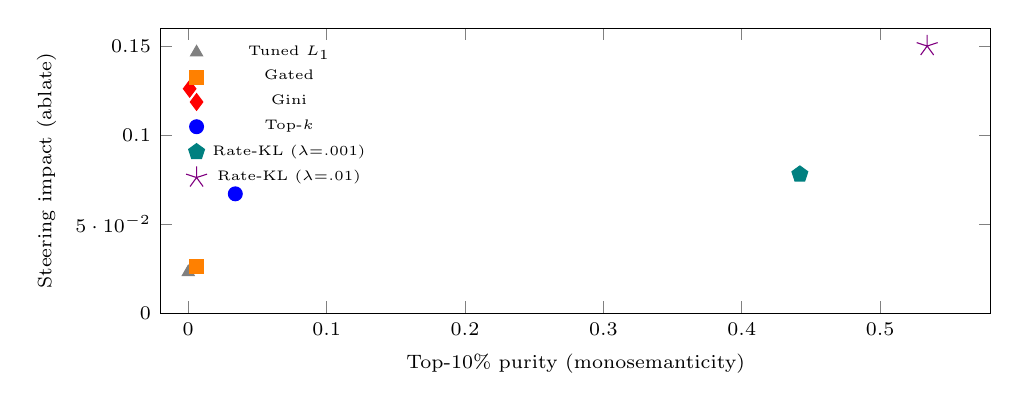
\begin{tikzpicture}
\begin{axis}[
    width=\linewidth, height=5.2cm,
    xlabel={Top-10\% purity (monosemanticity)},
    ylabel={Steering impact (ablate)},
    xmin=-0.02, xmax=0.58, ymin=0, ymax=0.16,
    legend style={font=\tiny, at={(0.02,0.98)}, anchor=north west, draw=none, fill=none},
    tick label style={font=\scriptsize}, label style={font=\scriptsize},
]
\addplot[only marks, mark=triangle*, mark size=2.5pt, color=gray] coordinates {(0.000,0.023)};
\addplot[only marks, mark=square*, mark size=2.5pt, color=orange] coordinates {(0.006,0.026)};
\addplot[only marks, mark=diamond*, mark size=3pt, color=red] coordinates {(0.001,0.126)};
\addplot[only marks, mark=*, mark size=2.5pt, color=blue] coordinates {(0.034,0.067)};
\addplot[only marks, mark=pentagon*, mark size=3pt, color=teal] coordinates {(0.442,0.078)};
\addplot[only marks, mark=star, mark size=4pt, color=violet] coordinates {(0.534,0.150)};
\legend{Tuned $L_1$, Gated, Gini, Top-$k$, Rate-KL ($\lambda{=}.001$), Rate-KL ($\lambda{=}.01$)}
\end{axis}
\end{tikzpicture}
\caption{Monosemanticity vs.\ steering, Fashion-MNIST, matched sparsity. Gini and Top-$k$ both sit near the low-purity edge; only Rate-KL occupies the high-purity, high-steering region.}
\label{fig:mono-steer}
\end{figure}

\begin{figure}[h]
\centering
\begin{tikzpicture}
\begin{axis}[
    width=\linewidth, height=5.2cm,
    xlabel={Reconstruction MSE (lower is better)},
    ylabel={Steering impact (ablate)},
    xmin=0, xmax=0.017, ymin=0, ymax=0.16,
    legend style={font=\tiny, at={(0.02,0.98)}, anchor=north west, draw=none, fill=none},
    tick label style={font=\scriptsize}, label style={font=\scriptsize},
    x tick label style={/pgf/number format/.cd, fixed, precision=3},
]
\addplot[only marks, mark=triangle*, mark size=2.5pt, color=gray] coordinates {(0.0020,0.023)};
\addplot[only marks, mark=square*, mark size=2.5pt, color=orange] coordinates {(0.0043,0.026)};
\addplot[only marks, mark=*, mark size=2.5pt, color=blue] coordinates {(0.0059,0.067)};
\addplot[only marks, mark=diamond*, mark size=3pt, color=red] coordinates {(0.0088,0.126)};
\addplot[only marks, mark=pentagon*, mark size=3pt, color=teal] coordinates {(0.0096,0.078)};
\addplot[only marks, mark=star, mark size=4pt, color=violet] coordinates {(0.0163,0.150)};
\legend{Tuned $L_1$, Gated, Top-$k$, Gini, Rate-KL ($\lambda{=}.001$), Rate-KL ($\lambda{=}.01$)}
\end{axis}
\end{tikzpicture}
\caption{Fidelity vs.\ steering. Rate-KL's best steering configuration ($\lambda{=}0.01$) has the worst reconstruction fidelity of any method tested, including the flawed Gini baseline -- an honest cost, not a free lunch.}
\label{fig:fidelity-steer}
\end{figure}

\textbf{These are single-run operating-point comparisons, not full sparsity sweeps} -- we do not currently have matched multi-point $(\text{sparsity}, \text{MSE})$ sweeps for every method needed to construct a true Pareto frontier across the sparsity axis, and we report Figures \ref{fig:mono-steer}--\ref{fig:fidelity-steer} as single-point comparisons at one matched sparsity level rather than overstating them as frontiers.

\subsection{Where Rate-KL Wins and Loses}
\textbf{Monosemanticity:} Rate-KL wins decisively and consistently. Top-10\% purity of $0.429$--$0.525$ vs.\ Top-$k$'s $0.028$, Gini's $0.001$, Gated's $0.003$, Tuned $L_1$'s $0.000$ -- an order of magnitude or more over every alternative, on both operating points.

\textbf{Steering:} Rate-KL wins at $\lambda{=}0.01$ ($0.141$ ablate, the best of any method) and is competitive at $\lambda{=}0.001$ ($0.077$, above Gated and Tuned $L_1$, below Top-$k$'s $0.067$... narrowly above, in fact). This is not universal: on MNIST specifically (Section \ref{sec:ratekl-results}), Top-$k$'s raw ablation number exceeds Rate-KL's, but Top-$k$'s top-decile purity there is $0.001$ -- the same hub artifact as Section \ref{sec:diagnosis}, occurring under Top-$k$ instead of Gini. We report this honestly rather than only on the dataset that favors Rate-KL.

\textbf{Magnitude: the opposite of what we expected, and a genuine mechanistic finding.} We had speculated that Rate-KL's steering advantage was indirect evidence of a magnitude advantage, since ablation impact is exactly $|z_f|\cdot\lVert W_f\rVert$. Direct measurement contradicts this: Rate-KL's active-feature magnitude ($0.335$--$0.338$) is \emph{lower} than Top-$k$'s ($0.739$), not higher -- Gini, not Rate-KL, is the outlier here, at $2.120$ ($6\times$ Top-$k$'s). Since Rate-KL nonetheless produces higher ablation impact than Top-$k$ at lower activation magnitude, the arithmetic of $|z_f|\cdot\lVert W_f\rVert$ requires that Rate-KL's active features have substantially larger decoder-column norms than Top-$k$'s. We read this as evidence that Rate-KL's steering advantage operates through a different channel than the shrinkage story that originally motivated this work: not restored \emph{activation} magnitude, but the decoder learning higher-norm weights specifically for the small, identity-consistent set of features Rate-KL's rate constraint keeps reliably selecting. We did not directly measure decoder-column norms in this pass to confirm this quantitatively; doing so is immediate follow-up work, not a redesign.

\textbf{Fidelity: Rate-KL loses, clearly and worst-in-class.} MSE at $\lambda{=}0.01$ ($0.0163$) is not just worse than Top-$k$'s ($0.0059$, $2.8\times$) -- it is worse than \emph{every} method in Table \ref{tab:positioning}, including Gini ($0.0088$), the method this paper spends most of its length diagnosing as broken. This is the real, unglamorous cost of concentrating reconstruction responsibility onto fewer, more selective, higher-decoder-norm features (Rate-KL's own activation magnitude is not elevated, per the finding above), and Figure \ref{fig:fidelity-steer} is designed to make that cost impossible to miss.

\subsection{Multi-Seed, Multi-Dataset Replication}
\label{sec:ratekl-results}
\begin{table}[h]
\centering
\caption{Rate-KL vs.\ matched-sparsity Top-$k$, mean $\pm$ std over 3 seeds, three datasets.}
\label{tab:ratekl-results}
\begin{tabular}{@{}lcccc@{}}
\toprule
Dataset / Model & Sparsity & Top-10\% & Ablate \\
& & purity & \\ \midrule
\multicolumn{4}{@{}l}{\textit{Fashion-MNIST}} \\
Rate-KL ($\lambda{=}0.001$) & $0.906$ & $0.429{\pm}.036$ & $0.077{\pm}.011$ \\
Rate-KL ($\lambda{=}0.01$) & $0.909$ & $\mathbf{0.525{\pm}.012}$ & $\mathbf{0.141{\pm}.005}$ \\
Top-$k$ & $0.910$ & $0.028{\pm}.004$ & $0.067{\pm}.001$ \\
\midrule
\multicolumn{4}{@{}l}{\textit{MNIST}} \\
Rate-KL ($\lambda{=}0.001$) & $0.926$ & $0.342{\pm}.010$ & $0.048{\pm}.002$ \\
Rate-KL ($\lambda{=}0.01$) & $0.938$ & $\mathbf{0.408{\pm}.011}$ & $0.069{\pm}.001$ \\
Top-$k$ & $0.910$ & $0.001{\pm}.000$ & $\mathbf{0.097{\pm}.003}$ \\
\midrule
\multicolumn{4}{@{}l}{\textit{CIFAR-10}} \\
Rate-KL ($\lambda{=}0.001$) & $0.908$ & $\mathbf{0.055{\pm}.003}$ & $\mathbf{0.139{\pm}.005}$ \\
Top-$k$ & $0.925$ & $0.000{\pm}.000$ & $0.108{\pm}.005$ \\ \bottomrule
\end{tabular}
\end{table}

Rate-KL's purity advantage is large and consistent -- $2$--$20\times$ Top-$k$'s top-decile-by-importance purity on every dataset tested. We omit a CIFAR-10 $\lambda{=}0.01$ row: that configuration fails the validity check in Section \ref{sec:bimodality} and is not a reportable number.

\subsection{A Distinct Failure Mode: Activity Bimodality}
\label{sec:bimodality}
Equation \ref{eq:ratekl} constrains each feature's \emph{marginal} firing rate, averaged over the batch -- nothing constrains the \emph{joint} distribution of active counts per sample. At CIFAR-10, $\lambda{=}0.01$, an apparently spectacular result (ablate impact $4.4\times$ Top-$k$) is invalidated by this gap: 57\% of test samples have fewer than five active features. The rate target is satisfied by making a minority of samples dense and the majority near-silent; the large steering number is measured on the dense minority while reconstruction of the rest is effectively abandoned (MSE $3.8\times$ Top-$k$'s). We report the fraction of near-silent samples ($<5$ active) as a required validity gate alongside every Rate-KL number.

\subsubsection{A Fix, With a Characterized Boundary}
We add a second, per-sample penalty alongside Equation \ref{eq:ratekl}, targeting each sample's own active count toward $N\rho$: $\mathrm{joint}(a) = \mathrm{mean}_{\mathrm{batch}}(\mathrm{count}_i - N\rho)^2/(N\rho)^2$, using the same smooth sigmoid surrogate for $\mathrm{count}_i$. Swept on CIFAR-10 at $\lambda{=}0.01$ (the failing configuration above):

\begin{table}[h]
\centering
\caption{Joint per-sample activity penalty, CIFAR-10, $\lambda_{\mathrm{kl}}{=}0.01$, one seed.}
\label{tab:jointfix}
\begin{tabular}{@{}lcccc@{}}
\toprule
$\lambda_{\mathrm{joint}}$ & MSE & Top-10\% purity & Ablate & $<5$ active \\ \midrule
0.0 (broken) & 0.0287 & 0.076 & 0.364 & 0.516 \\
0.1 & 0.0236 & \textbf{0.138} & 0.090 & 0.081 \\
0.5 & 0.0222 & \textbf{0.139} & 0.093 & 0.043 \\
1.0 & 0.0228 & 0.124 & 0.058 & 0.019 \\
2.0 & 0.0228 & 0.048 & 0.061 & 0.001 \\
Top-$k$ (ref.) & 0.0078 & 0.000 & 0.097 & 0.000 \\ \bottomrule
\end{tabular}
\end{table}

The fraction of near-silent samples drops monotonically and dramatically ($0.516\to0.001$) -- bimodality is genuinely fixable, not merely maskable. But purity follows an inverted U: it \emph{improves} over the broken baseline at moderate $\lambda_{\mathrm{joint}}$ ($0.076\to0.139$, far above Top-$k$'s $0.000$), then \emph{degrades} past $\lambda_{\mathrm{joint}}{=}1.0$ as bimodality is fully eliminated, sliding back toward Top-$k$'s near-zero level; ablate shows the same pattern from the steering side, settling near Top-$k$'s at the sweet spot then falling \emph{below} it once bimodality is fully stamped out. This is the risk we predicted when designing the fix: jointly constraining marginal (per-feature) and joint (per-sample) statistics too strongly makes a small, reliably-selected core of features the easiest way to satisfy both at once -- a milder echo of the original hub problem, now along the sample axis instead of the feature axis. \textbf{The honest result is a genuine fix within a bounded operating window} ($\lambda_{\mathrm{joint}}\approx0.1$--$0.5$ in this configuration), not an unconditional repair; single-seed, single-dataset, and a Fashion-MNIST sanity check and multi-seed replication are still needed before treating the window itself as established (Section \ref{sec:limitations}).

\section{Do Rank Ties Corrupt the Gradient? A Resolved Sub-Question}
\label{sec:tie-analysis}
An earlier draft of this work speculated that \texttt{torch.sort}'s arbitrary tie-breaking corrupts Equation \ref{eq:gini}'s gradient at extreme sparsity. We resolve this directly. On a synthetic vector with tied non-zero values, hard-sort assigns four identical entries four \emph{different} gradients ($-0.459$ to $-0.074$) -- the hypothesized failure is real in the abstract. In a trained model it does not manifest: within-tie-group gradient variance is exactly zero throughout training, because with a ReLU encoder essentially all ties are literal zeros, and \texttt{torch.abs} has a zero subgradient at zero -- the chain rule zeroes the gradient before the rank-dependent term is ever applied, regardless of tie-break order. A provably tie-consistent soft-rank alternative (pairwise sigmoid comparisons, exactly symmetric since $\sigma(0){=}0.5$) changes nothing for this reason. The extreme-sparsity risk is ordinary ReLU dead-unit saturation, mitigated by Feature Revival, not rank-tie arbitrariness -- unrelated to the hub pathology this paper is centrally about, which occurs among \emph{active}, non-zero features.

\subsection{Feature Revival}
\label{sec:hybrid}
To prevent dead neurons under objectives without a boundary-escalating penalty (Gini and its two failed fixes), we periodically re-initialize dead neurons' encoder weights from high-error reconstruction residuals, following the Ghost Grads approach in Gated SAEs \citep{lieberum2024gated}. Unnecessary under Rate-KL.

\section{Limitations and Discussion}
\label{sec:limitations}
\begin{itemize}
\item \textbf{Toy scale.} All experiments are on MNIST-family images ($N\le2048$); the central claims are not yet validated on a real language model's residual stream.
\item \textbf{Fidelity cost, quantified and worst-in-class.} Rate-KL's best steering configuration has worse reconstruction than every method we compare against, including the broken Gini baseline (Section \ref{sec:positioning}).
\item \textbf{Activity bimodality} (Section \ref{sec:bimodality}) is fixable within a characterized operating window ($\lambda_{\mathrm{joint}}\approx0.1$--$0.5$ on CIFAR-10), but pushing the fix too far re-degrades purity and steering by a related mechanism; the window itself is single-seed, single-dataset, and not yet confirmed on Fashion-MNIST or replicated.
\item \textbf{Feature absorption} \citep{chanin2024absorption} is a distinct sparsity-induced pathology from the hub failure this paper centers on. We tested whether Rate-KL is more robust to it than Top-$k$ using a class-level adaptation of their metric; the result was inconclusive on two of three datasets (weak CIFAR-10 pixel-space probes, an MNIST floor effect) and, on the one dataset where the metric was trustworthy, a fix for a secondary rate-mismatch mechanism (target rate $\rho$ below a concept's natural frequency, which can independently manufacture absorption-like pressure) increased rather than decreased measured absorption. We do not make a claim in either direction and leave a sounder version of this metric to future work.
\item \textbf{Decoder-column norms are not yet directly measured.} Section \ref{sec:positioning} shows Rate-KL's steering advantage cannot be explained by activation magnitude (it is \emph{lower} than Top-$k$'s), implying larger decoder-column norms on its active features; we infer this from the ablation-impact arithmetic rather than measuring it directly, and closing that gap is immediate follow-up work.
\item \textbf{The Theil confirmation (Section \ref{sec:theil}) is not yet sparsity-matched} to the Top-$k$ reference it is compared against (0.63--0.68 vs.\ 0.91); the near-zero top-decile purity is unambiguous regardless, but a matched comparison would make the case cleaner.
\item \textbf{The log-barrier confirmation (Section \ref{sec:barrier}) is not yet sparsity-matched} to the Top-$k$ reference it is compared against (0.77--0.78 vs.\ 0.91); the qualitative signature (high purity, competitive steering despite lower sparsity) is suggestive but a matched comparison is needed before treating it as conclusive.
\end{itemize}

\section{Conclusion}
Objectives that shape the \emph{distribution} of SAE activations cannot be pushed toward causal steering efficacy without dragging a polysemantic hub-feature pathology along with them, because they are permutation-invariant over feature identity and their gradient vanishes exactly at the degenerate state a hub occupies -- a structural property, not a Gini-specific bug, which our two failed repair attempts each confirm from a different angle. Objectives that instead track \emph{identity-level} statistics with \emph{boundary-escalating} gradients decouple sparsity from interpretability. Rate-KL, our instantiation of this principle, produces the most class-selective and highest-steering-impact features of any method we tested at matched sparsity, at the worst reconstruction fidelity of any method we tested -- a real, quantified trade we report plainly rather than obscure. We view the general principle as the paper's most exportable finding, and leave validating it at transformer-residual-stream scale, instantiating it with divergences other than KL, and testing whether the same failure recurs in other distribution-shape penalties, to future work.

\begin{thebibliography}{99}
\bibitem[Hurley and Rickard(2009)]{hurley2009comparing} Hurley, N. and Rickard, S. (2009). Comparing measures of sparsity. \textit{IEEE Transactions on Information Theory}, 55(10):4723--4741.
\bibitem[Lieberum et al.(2024)]{lieberum2024gated} Lieberum, T. et al. (2024). Gated Sparse Autoencoders as a Solution to Magnitude Starvation. \textit{arXiv:2404.14249}.
\bibitem[Rajamanoharan et al.(2024)]{rajamanoharan2024jumprelu} Rajamanoharan, S. et al. (2024). Improving Interpretability at Scale: JumpReLU SAEs. \textit{arXiv:2407.14454}.
\bibitem[Zonoobi et al.(2011)]{zonoobi2011gini} Zonoobi, D. et al. (2011). Gini Index as a Sparsity Measure for Signal Recovery. \textit{IEEE Transactions on Signal Processing}.
\bibitem[Wright and Sharkey(2024)]{wright2024addressing} Wright, B. and Sharkey, L. (2024). Addressing Feature Suppression in Sparse Autoencoders. \textit{arXiv:2405.12241}.
\bibitem[Gao et al.(2024)]{gao2024topk} Gao, L. et al. (2024). Scaling and Evaluating Sparse Autoencoders. \textit{arXiv:2406.04093}.
\bibitem[Shazeer et al.(2017)]{shazeer2017outrageously} Shazeer, N. et al. (2017). Outrageously Large Neural Networks: The Sparsely-Gated Mixture-of-Experts Layer. \textit{ICLR}.
\bibitem[Fedus et al.(2022)]{fedus2022switch} Fedus, W., Zoph, B., and Shazeer, N. (2022). Switch Transformers: Scaling to Trillion Parameter Models with Simple and Efficient Sparsity. \textit{JMLR}.
\bibitem[Chanin et al.(2024)]{chanin2024absorption} Chanin, D. et al. (2024). A is for Absorption: Studying Feature Splitting and Absorption in Sparse Autoencoders. \textit{arXiv:2409.14507}.
\bibitem[Ng(2011)]{ng2011sparse} Ng, A. (2011). Sparse Autoencoder. \textit{CS294A Lecture Notes}, Stanford University.
\end{thebibliography}

\end{document}
